\documentclass[12pt]{article}
\usepackage{amscd,amssymb,amsthm,amsxtra,exscale,latexsym,verbatim,paralist}
\usepackage{mathrsfs}
\usepackage[T1]{fontenc}
\usepackage{newtxmath,newtxtext}
\usepackage[left = 2cm, top = 2cm, bottom = 2cm, right = 2cm]{geometry}

\usepackage{hyperref}
\usepackage{tikz}
\usetikzlibrary{patterns}

\newcommand{\XB}{\color{black}}
\newcommand{\XBB}{\color{blue}}
\newcommand{\XV}{\color{violet}}
\newcommand{\XR}{\color{red}}
\newcommand{\ds}{\displaystyle}

\setlength{\parindent}{0pt} 
\setlength{\parskip}{\baselineskip}

\theoremstyle{plain}
\newtheorem{ex}{Exercise}

\renewcommand{\proofname}{Solution}

\begin{document}

\title{\textbf{MTH385}: History of Mathematics - Homework \#6}
\date{\today}
\author{\XV\textit{\large{\href{https://github.com/casonk}{Cason Konzer}}}\XB}

\maketitle

\hrulefill

\newpage
%%%%%%%%%%%%%%%%%%%%%%%%%%%%%%%%%%%%%%%%%%%%%%%%%%%%%%%%%%%%%%%%%%%%%%%%%%%%%%%%%%%%%%%%%%%%%%%%%%%%%%%%%%%%%
%%%%%%%%%%%%%%%%%%     #1     %%%%%%%%%%%%%%%%%%%%%%%%%%%%%%%%%%%%%%%%%%%%%%%%%%%%%%%%%%%%%%%%%%%%%%%%%%%%%%%
%%%%%%%%%%%%%%%%%%%%%%%%%%%%%%%%%%%%%%%%%%%%%%%%%%%%%%%%%%%%%%%%%%%%%%%%%%%%%%%%%%%%%%%%%%%%%%%%%%%%%%%%%%%%%

\XBB\hrulefill\XB \\
\begin{ex} [3.5.1]
  Explain the solution $ x = 21 / 4 $, $ y = 71 / 8 $ to $ x^{3} - 3x^{2} + 3x + 1 = y^{2} $ given by Diophantus (Heath~(1910), p. 242) by constructing the tangent through the obvious rational point on this curve.
\end{ex}

\begin{center}
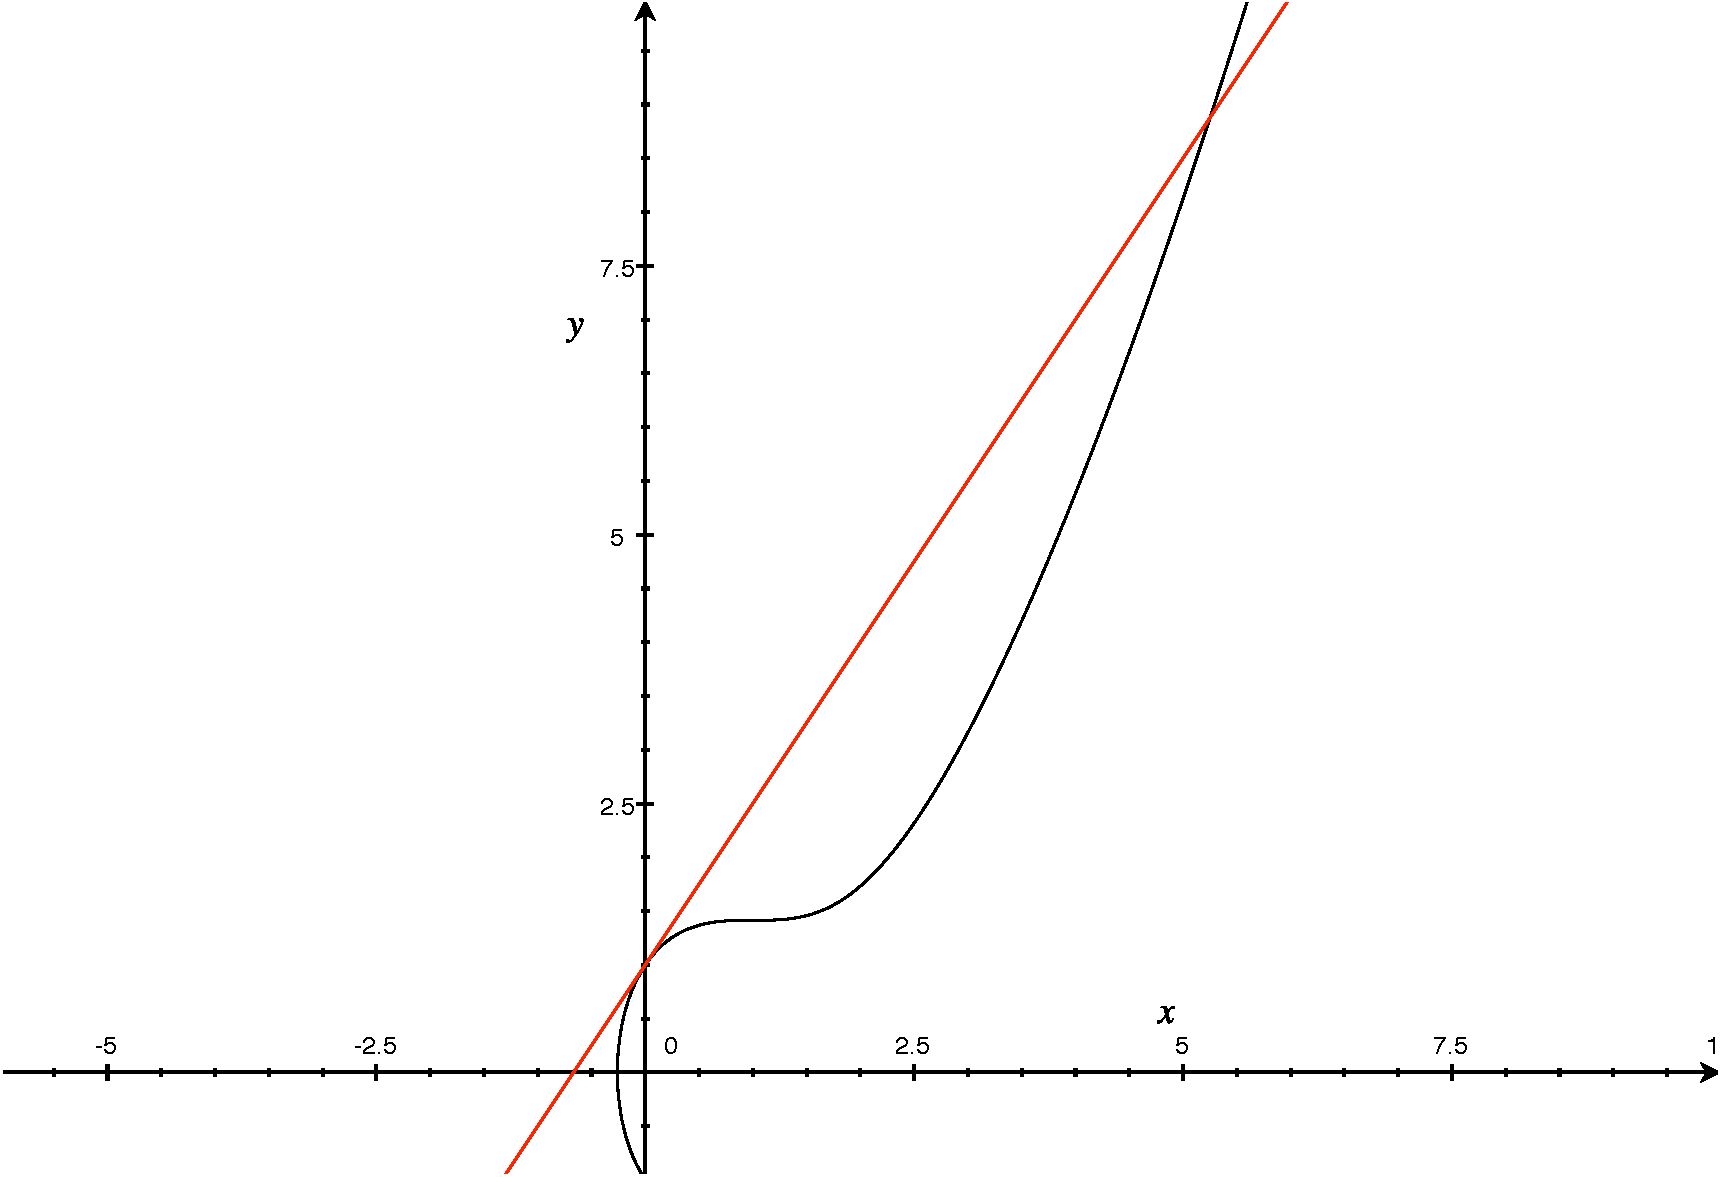
\includegraphics[scale=0.6]{cubic}

Figure~3.4: Cubic curve $y^2=x^3-3x^2+3x+1$ and tangent
\end{center}
\XBB\hrulefill\XB \\

\newpage

\begin{proof}
  \ \\

  We can see that the obvious rational point exists at $ (x, y) = (0, 1) $.

  From this point we will construct the tangent. 

  \begin{itemize}
    \item $ \ds \frac{dy}{dx} 2y = 3x^{2} - 6x + 3 $.
    \item $ \ds \frac{dy}{dx} = (3x^{2} - 6x + 3) / 2y $.
    \item $ \ds \frac{dy}{dx} = (3(0)^{2} - 6(0) + 3) / 2(1) = 3 / 2 $.
  \end{itemize}

  We can thus see that the tangent line takes $ (y - 1) = 3(x - 0) / 2 \Rightarrow y = 3x/2 + 1 $. 

  Substituting our tangent into the cubic we find \dots

  \begin{itemize}
    \item $ \ds x^{3} - 3x^{2} + 3x + 1 = (3x/2 + 1)^{2} = 9x^{2}/4 + 3x + 1 $.
    \item $ \ds x^{3} - 3x^{2} = 9x/4 \Rightarrow x^{2}(x - 3 - 9/4) = 0 $.
    \item The obvious solution is $ x = 0 $; Consider $ x - 21/4 = 0 $.
    \item As expected $ x = 21/4 $. 
    \item Solving for $ y \ ; \ y = 3(21/4)/2 + 1 = 63/8 + 1 = 71/8 $.
  \end{itemize} 

  Diophantus found this solution by first finding an obvious rational solution, and then constructing the tangent, with rational slope, 
  to find a second rational solution at the intersection of the tangent and the cubic. 

\end{proof}

\newpage
%%%%%%%%%%%%%%%%%%%%%%%%%%%%%%%%%%%%%%%%%%%%%%%%%%%%%%%%%%%%%%%%%%%%%%%%%%%%%%%%%%%%%%%%%%%%%%%%%%%%%%%%%%%%%
%%%%%%%%%%%%%%%%%%     #2     %%%%%%%%%%%%%%%%%%%%%%%%%%%%%%%%%%%%%%%%%%%%%%%%%%%%%%%%%%%%%%%%%%%%%%%%%%%%%%%
%%%%%%%%%%%%%%%%%%%%%%%%%%%%%%%%%%%%%%%%%%%%%%%%%%%%%%%%%%%%%%%%%%%%%%%%%%%%%%%%%%%%%%%%%%%%%%%%%%%%%%%%%%%%%

\XBB\hrulefill\XB \\
\begin{ex} [3.5.2]
  Rederive the following rational point construction of Vi\`{e}te~(1593), p. 145. Given the rational point $ (a, b) $ on $ x^{3} - y^{3} = a^{3} - b^{3} $ , show that the tangent at $(a,b)$ is
  \[
    y = \frac{a^{2}}{b^{2}}(x - a) + b
  \]
  \centering and that the other intersection of the tangent with the curve is the rational point
  \[
    x = a\frac{a^{3} - 2b^{3}}{a^{3} + b^{3}}, \qquad y = b\frac{b^{3} - 2a^{3}}{a^{3} + b^{3}}.
  \]
\end{ex}
\XBB\hrulefill\XB \\

\begin{proof}
  \ \\

  From the given point we will construct the tangent. 

  \begin{itemize}
    \item $ \ds y^{3} = x^{3} + b^{3} - a^{3} $.
    \item $ \ds \frac{dy}{dx} 3y^{2} = 3x^{2} $.
    \item $ \ds \frac{dy}{dx} = 3x^{2} / 3y^{2} $.
    \item $ \ds \frac{dy}{dx} = (a)^{2} / (b)^{2} $.
  \end{itemize}

  We can thus see that the tangent line takes $ (y - b) = a^{2} / b^{2} (x - a) \Rightarrow y = a^{2}(x - a) / b^{2}  + b $. 

  Substituting the given intersections into our tangent we find \dots

  \begin{itemize}
    \item $ \ds b\frac{b^{3} - 2a^{3}}{a^{3} + b^{3}} = a^{2}(a\frac{a^{3} - 2b^{3}}{a^{3} + b^{3}} - a) / b^{2}  + b $.
    \item $ \ds \frac{b^{4} - 2ba^{3}}{a^{3} + b^{3}} = \frac{a^{6} - 2a^{3}b^{3}}{a^{3}b^{2} + b^{5}} - a^{3}/b^{2} + b = \frac{a^{6} - 2a^{3}b^{3}}{a^{3}b^{2} + b^{5}} - \frac{a^{6} + a^{3}b^{3}}{a^{3}b^{2} + b^{5}} + \frac{a^{3}b^{3} + b^{6}}{a^{3}b^{2} + b^{5}} $.
    \item $ \ds \frac{b^{4} - 2ba^{3}}{a^{3} + b^{3}} = \frac{b^{6} - 2a^{3}b^{3}}{a^{3}b^{2} + b^{5}} ; $ Which holds.   
    \item Thus the given $ (x, y) $ lie on both the tangent to the know rational point and the original curve.

  \end{itemize} 

\end{proof}

\newpage

The \emph{Jade Mirror of Four Unknowns} does not go beyond four equations in four unknowns (hence the name). The idea is quite general, but it becomes hard to implement on the counting board when there are more than four unknowns. An amusing problem in three unknowns from the \emph{Jade Mirror}, which does not require the full strength of the elimination method, is given in the exercises below.

%%%%%%%%%%%%%%%%%%%%%%%%%%%%%%%%%%%%%%%%%%%%%%%%%%%%%%%%%%%%%%%%%%%%%%%%%%%%%%%%%%%%%%%%%%%%%%%%%%%%%%%%%%%%%
%%%%%%%%%%%%%%%%%%     #3     %%%%%%%%%%%%%%%%%%%%%%%%%%%%%%%%%%%%%%%%%%%%%%%%%%%%%%%%%%%%%%%%%%%%%%%%%%%%%%%
%%%%%%%%%%%%%%%%%%%%%%%%%%%%%%%%%%%%%%%%%%%%%%%%%%%%%%%%%%%%%%%%%%%%%%%%%%%%%%%%%%%%%%%%%%%%%%%%%%%%%%%%%%%%%

\XBB\hrulefill\XB \\
\begin{ex} [5.2.4]
  Problem~2 in the Jade Mirror (see Hoe~(1977), p. 135) is to find the side $ a $ of a right-angled triangle $ (a, b, c) $ such that
  \begin{align*}
    a^{2} - (b + c - a) &= ab, \\
    b^{2} + (a + c - b) &= bc.
  \end{align*}
  \centering The \emph{Jade Mirror} suggests choosing the unknowns $ x = a $ and $ y = b + c $. Using $ a^{2} = c^{2} - b^{2} $, show that this implies
  \begin{align*}
    b &= (y - x^{2} / y) / 2, \\
    c &= (y + x^{2} / y) / 2.
  \end{align*}
\end{ex}
\XBB\hrulefill\XB \\

\begin{proof}
  \ \\

  From the given we have \dots

  \begin{itemize}
    \item $ \ds a = x, \quad a^{2} = x^{2} $.
    \item $ \ds b = y - c, \quad b^{2} = y^{2} - 2yc + c^{2} $.
    \item $ \ds a^{2} + b^{2} = c^{2} \Rightarrow x^{2} + y^{2} - 2yc + c^{2} = c^{2} \Rightarrow x^{2} + y^{2} - 2yc = 0 $.
    \item Solving for $ c $ we find \dots
    \item $ \ds 2yc = x^{2} + y^{2} \Rightarrow c = (x^{2} + y^{2}) / 2y = (y + x^{2} / y) / 2 $.
    \item We can now solve for $ b $ \dots
    \item $ \ds b = y - c = y - (x^{2} + y^{2}) / 2y = (2y^{2} - x^{2} + y^{2}) / 2y = (y^{2} - x^{2}) / 2y = (y - x^{2} / y) / 2 $. 
  \end{itemize}

  We can see the implicaton follows from our assumption. 

\end{proof}

\newpage
%%%%%%%%%%%%%%%%%%%%%%%%%%%%%%%%%%%%%%%%%%%%%%%%%%%%%%%%%%%%%%%%%%%%%%%%%%%%%%%%%%%%%%%%%%%%%%%%%%%%%%%%%%%%%
%%%%%%%%%%%%%%%%%%     #4     %%%%%%%%%%%%%%%%%%%%%%%%%%%%%%%%%%%%%%%%%%%%%%%%%%%%%%%%%%%%%%%%%%%%%%%%%%%%%%%
%%%%%%%%%%%%%%%%%%%%%%%%%%%%%%%%%%%%%%%%%%%%%%%%%%%%%%%%%%%%%%%%%%%%%%%%%%%%%%%%%%%%%%%%%%%%%%%%%%%%%%%%%%%%%

\XBB\hrulefill\XB \\
\begin{ex} [5.2.5]
  Deduce that the first two equations in Exercise~5.2.4 are equivalent, respectively, to
  \begin{align*}
    (-2 - x)y^{2} + (2x + 2x^{2})y + x^{3} &= 0 \\
    (2 - x)y^{2} + 2xy + x^{3} &= 0.
  \end{align*}
\end{ex}
\XBB\hrulefill\XB \\

\begin{proof}
  \ \\

  We will solve but substitution \dots

  Tackling the first equation ` $ a^{2} - (b + c - a) = ab $ '

  \begin{itemize}
    \item $ \ds a^{2} - (b + c - a) - ab = x^{2} - (y - x) - x(y - x^{2} / y) / 2 = 0 $.
    \item $ \ds 2x^{2} - 2y + 2x - x(y - x^{2} / y) = 2x^{2} - 2y + 2x - xy + x^{3} / y =  0 $.
    \item $ \ds 2x^{2}y - 2y^{2} + 2xy - xy^{2} + x^{3} = (-2 - x)y^{2} + (2x + 2x^{2})y + x^{3} = 0 $.
  \end{itemize}

  Tackling the second equation ` $ b^{2} + (a + c - b) = bc $ '

  \begin{itemize}
    \item $ \ds b^{2} + (a + c - b) - bc = 0 $.
    \item $ \ds ((y - x^{2} / y) / 2)^{2} + (x + (y + x^{2} / y) / 2 - (y - x^{2} / y) / 2) - ((y - x^{2} / y) / 2)((y + x^{2} / y) / 2) = 0 $.
    \item $ \ds (y^{2} - 2x^{2} + x^{4} / y^{2}) / 4 + (x + (2x^{2} / y) / 2) - (y^{2} - x^{4} / y^{2}) / 4 = 0 $.
    \item $ \ds y^{2} - 2x^{2} + x^{4} / y^{2} + 4x + 4x^{2} / y - y^{2} + x^{4} / y^{2} = - 2x^{2} + x^{4} / y^{2} + 4x + 4x^{2} / y + x^{4} / y^{2} = 0 $.
    \item $ \ds -2xy^{2} + 4y^{2} + 4xy + 2x^{3} = 0 $.
    \item $ \ds -xy^{2} + 2y^{2} + 2xy + x^{3} = (2 - x)y^{2} + 2xy + x^{3} = 0 $.
  \end{itemize}
  
  We can now see the first two equations are equivalent, respectively.

\end{proof}

\newpage
%%%%%%%%%%%%%%%%%%%%%%%%%%%%%%%%%%%%%%%%%%%%%%%%%%%%%%%%%%%%%%%%%%%%%%%%%%%%%%%%%%%%%%%%%%%%%%%%%%%%%%%%%%%%%
%%%%%%%%%%%%%%%%%%     #5     %%%%%%%%%%%%%%%%%%%%%%%%%%%%%%%%%%%%%%%%%%%%%%%%%%%%%%%%%%%%%%%%%%%%%%%%%%%%%%%
%%%%%%%%%%%%%%%%%%%%%%%%%%%%%%%%%%%%%%%%%%%%%%%%%%%%%%%%%%%%%%%%%%%%%%%%%%%%%%%%%%%%%%%%%%%%%%%%%%%%%%%%%%%%%

\XBB\hrulefill\XB \\
\begin{ex} [5.2.6]
  By subtracting one equation in Exercise~5.2.5 from the other, deduce that $y=x^2/2$. Substitute this back to obtain a quadratic equation for $x$, with solution $x=a=4$. What are the values of $b$ and $c$?
\end{ex}
\XBB\hrulefill\XB \\

\begin{proof}
  \ \\

  Note first that $ 0 - 0 = 0 $. 

  \begin{itemize}
    \item $ \ds (-2 - x)y^{2} + (2x + 2x^{2})y + x^{3} - (2 - x)y^{2} - 2xy - x^{3} = 0 $. 
    \item $ \ds 2x^{2}y - 4y^{2} = 2y(x^{2} - 2y) = 0 $. 
    \item $ \ds y = 0, \quad y = x^{2} / 2$.
  \end{itemize}

  As $ y = 0 $ is a trivial solution, we are concerned with $ y = x^{2}/2 $. 

  By substitution we can find $ x $. 

  \begin{itemize}
    \item $ \ds (2 - x)y^{2} + 2xy + x^{3} = (2 - x)(x^{2}/2)^{2} + 2x(x^{2}/2) + x^{3} = 0 $.
    \item $ \ds (2 - x)(x^{4}/4) + x^{3} + x^{3} = x^{4}/2 - x^{5}/4 + 2x^{3} = 0 $.
    \item $ \ds 2x^{4} - x^{5} + 8x^{3} = -x^{3}(x^{2} -2x - 8) = x^{3}(x + 2)(x - 4) = 0 $.
    \item $ \ds x = 0, \quad x = -2, \quad x = 4 $.
  \end{itemize}

  As $ x = 0 $ is a trivial solution, and we do not allow negative lengths, we are concerned with $ x = 4 = a $. 

  We can now find the values of $ b $ and $ c $.

  \begin{itemize}
    \item $ \ds x^{2}/y = 2x^{2}/x^{2} = 2 $.
    \item $ \ds (y - x^{2} / y) / 2 = (x^{2}/2 - 2) / 2 = x^{2}/4 - 1 $.
    \item $ \ds b = 4^{2}/4 - 1 = 4 - 1 = 3 $.
    \item $ \ds (y + x^{2} / y) / 2 = (x^{2}/2 + 2) / 2 = x^{2}/4 + 1 $.
    \item $ \ds c = 4^{2}/4 + 1 = 4 + 1 = 5 $.
  \end{itemize}


\end{proof}


\end{document}

